% gjilguid2e.tex
% V2.0 released 1998 December 18
% V2.1 released 2003 October 7 -- Gregor Hutton, updated the web address for the style files.


% \documentclass[extra,mreferee]{gji} % one-column with extra.sty; see gji.cls
\documentclass[extra]{gji} % refer to gji.cls; two-column with extra.sty
% amsmath,amssymb
% \usepackage{natbib}
% \usepackage{timet,color} # has to be disabled to make gji extra correctly format the volume number and subtitles bold.
\usepackage[urlcolor=blue,citecolor=black,linkcolor=black]{hyperref}
\usepackage{graphicx} % to enable includegraphics[]{...}
\usepackage{amsmath} % for latex math
% \usepackage[authoryear,round,longnamesfirst]{natbib}
% \usepackage[utf8]{inputenc}% \usepackage{natbib} % use this package causes error
% \usepackage[english]{babel}

\bibliographystyle{gji}
% \bibliographystyle{apalike}
% \bibliographystyle{gji} % use gji.bst
% There are a lot of error using gji.bst to generate the main.bbl file, so I temporarily use the built-in apalike bibliography style.
% After the article is finished, generate the .bbl file with \bibliographystyle{gji}, then copy the \thebibliography section inside and manually fix all the error, and replace \bibliography{main} by this modified \begin{thebibliography}{}...\end{thebibliography} section (i.e. delete \bibliography{main} and put the \thebibliography section right before \label{lastpage} and \end{document}.





\usepackage{gji_extra} % This is superfluous. See at the end of gji.cls
% \usepackage{url}
% \usepackage{hyperref}
% \usepackage[english]{babel}

\usepackage{lineno} % applied in 2022-10-05


% \begin{document}
\title[Geophys.\ J.\ Int.: A Stochastic Model for Earthquake Rupture]
  {A Stochastic Model for Earthquake Rupture}
% \author[B.L.N. Kennett]
%   {B.L.N. Kennett$^1$\thanks{Pacific Region Office, GJI} \\
%   $^1$ Research School of Earth Sciences, Australian National
%     University, Canberra ACT \emph{0200}, Australia
%   }


\author[T.-H. Wu et al.]
  {T.-H. Wu$^1$ \thanks{tsung.hsi@g.ncu.edu.tw},
    C.-C. Chen$^{1,2}$ \thanks{chienchih.chen@g.ncu.edu.tw} and
    J.-H. Wang$^{1,3}$ \thanks{jhwang@earth.sinica.edu.tw}\\
  $^1$ Department of Earth Sciences, National Central University -  Zhongli  \emph{32001}, Taiwan\\
  $^2$ Earthquake-Disaster\ \& Risk Evaluation and Management Center, National Central University - Zhongli \emph{32001}, Taiwan \\
  $^3$  Institute of Earth Sciences, Academia Sinica - Nangang, \emph{11529}, Taiwan
  }


\date{Received YYYY Month DD; in original form YYYY Month DD}
\pagerange{\pageref{firstpage}--\pageref{lastpage}}
\volume{XXX}
\pubyear{YYYY}

%\def\LaTeX{L\kern-.36em\raise.3ex\hbox{{\small A}}\kern-.15em
%    T\kern-.1667em\lower.7ex\hbox{E}\kern-.125emX}
%\def\LATeX{L\kern-.36em\raise.3ex\hbox{{\Large A}}\kern-.15em
%    T\kern-.1667em\lower.7ex\hbox{E}\kern-.125emX}
% Authors with AMS fonts and mssymb.tex can comment out the following
% line to get the correct symbol for Geophysical Journal International.
% \let\leqslant=\leq

\newtheorem{theorem}{Theorem}[section]

\begin{document}

\label{firstpage}

\maketitle
\linenumbers % with \usepackage{lineno}
% KEYNOTE: EVERY \begin{equation} should be preceded by a blank line; otherwise, \linenumbers cannot properly works at the paragraph around it.

\begin{summary}
    Analytical solutions for the dynamics of an asymmetric many-body system are impossible to obtain in practice, and numerical solutions usually exhibit chaotic behaviors if interactions between bodies are considered.
    To resolve these problems, stochastic approaches have been extensively applied to model the dynamics of many-body systems.
    Following Langevin's approach, we propose a stochastic dynamic model for the earthquake rupture process, where the number of degrees of freedom is reduced by introducing a random force that accounts for the collision of structures and uncertainties in the heterogeneity of faulting planes.
    By regarding the tectonic process as a Coulomb friction process, the proposed Langevin equation can be understood as a stochastic variety of Newton's second law, giving the equation physical meaning by realizing stochastic processes as sample paths.
    
    For every Langevin equation, there is a corresponding partial differential equation known as the Fokker--Planck equation (FPE), which
    is mathematically equivalent to the Langevin equation but characterizes the same dynamics at the level of a probability function distribution.
    By leveraging the advantages of both equations, we obtain the theoretical rupture slip distribution by analytically solving the FPE and acquire the energy--duration relationship of synthetic events that are numerically generated according to the Langevin equation.
    
    The results of numerical simulations suggest a universal energy--duration scaling relationship, and
    the analytical and numerical solutions both coincide with the truncated exponential distribution empirically characterized by the rupture models of large earthquake events worldwide.
    Thus,
    we are able to relate the scaling parameter in the truncated exponential model to the ratio of the diffusion coefficient to the friction parameter in the Langevin equation under the condition of a large external driving force.
    
\end{summary}

\begin{keywords}
    %  \LaTeXe\ -- class files: \verb"gji.cls"\ -- sample text -- user guide.
    earthquake rupture -- friction process -- stochastic dynamics -- Langevin equation
    
\end{keywords}

\section{Introduction}

Earthquakes can be realized under the framework of Coulomb friction model as stick-slip frictional instabilities, which are fracture-like phenomena occurring on a non-uniform prestressed interface \citep{albertiniStochasticPropertiesStatic2020}.
The stick-slip explanation of earthquake can be dated back to \citet{braceStickSlipMechanismEarthquakes1966} who considered earthquakes as transitory phenomena that are subject to the long-term occurrence of friction within the Earth's crust.
As reviewed by \citet{scholzMechanicsEarthquakesFaulting1990}, friction (namely, Coulomb friction) is the product of various types of interactions between geometric structures on the two contacting interfaces.
In \citet{haessigModelingSimulationFriction1991}, Coulomb friction is further realized as the macroscopic phenomenon comprising multitude of successive and repetitive stick-slip events.


\section{Stochastic dynamics for heterogeneous friction}

Hence, the steady-state solution is

\begin{equation}
    P_\text{st}(v) = P_0\exp\left(\frac{F_\text{ext}v}{D}\right) \exp\left(\frac{-F_C v \frac{v}{|v|}}{D}\right),
    \label{Eq_Pst_a}
\end{equation}
% > Refer to that in matlab (GJI_2020.m).
or simply

\begin{equation}
    P_\text{st}(v) =
    \begin{cases}
        P_0 \exp{\left( \frac{F_\text{ext}+F_C}{D} v \right)} \text{, for } v\leq 0 \\
        P_0 \exp{\left( \frac{F_\text{ext}-F_C}{D} v \right)} \text{, for } v>0
    \end{cases}
    \label{Eq_Pst_b}
\end{equation}

\section{Results}
\subsection{The empirical distribution of rupture slips}

\begin{figure*}
    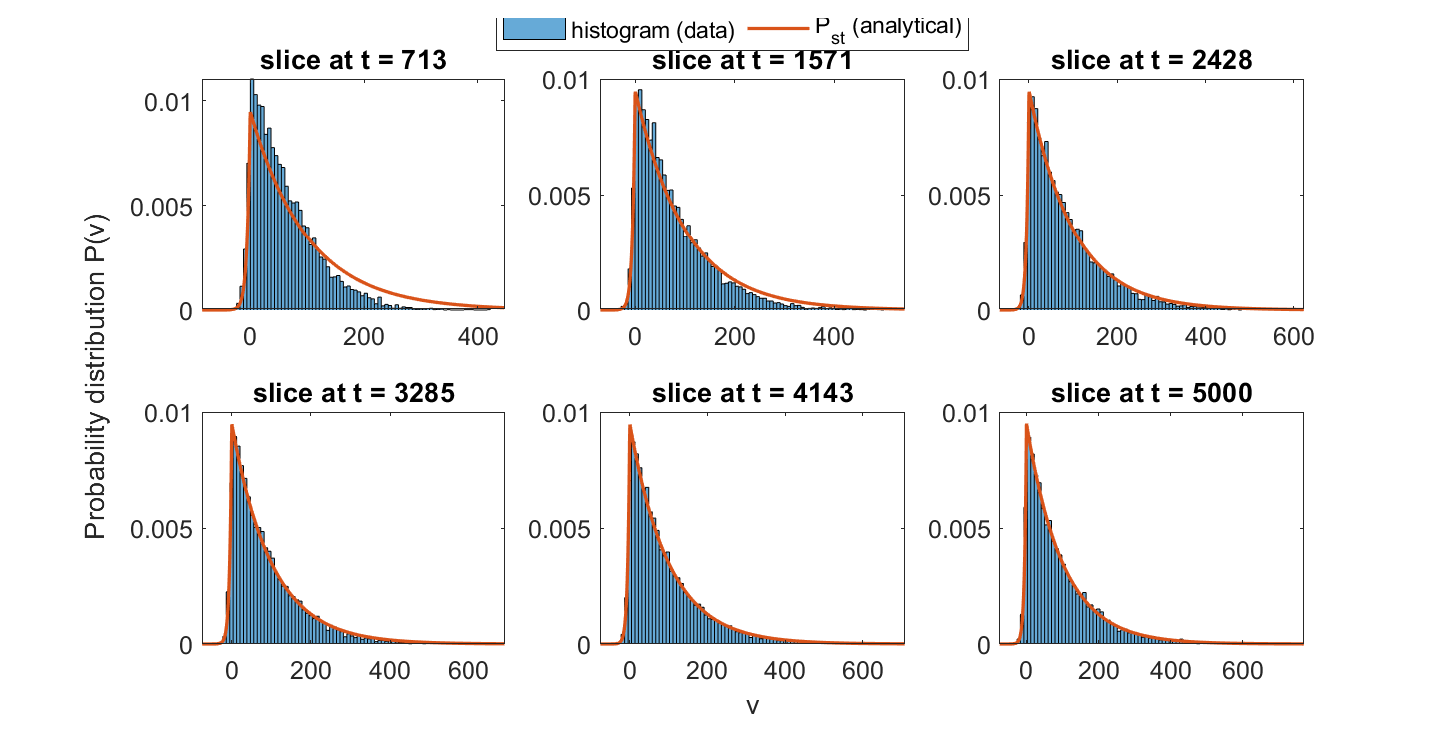
\includegraphics[width=\textwidth]{PstSlices_D[10]_r[1]_Fc[0.9].eps}
    % \vspace{5.5cm}
    \caption{The probability distribution of slip velocity calculated from an ensemble of samples sampled from total $10^4$ realizations at different time (the histogram), and the steady-state solution $P_\text{st}(v)$ (see Eq.\ref{Eq_Pst_a} and \ref{Eq_Pst_b}) (the red curve), in which $D=10$, $F_C=1$, $F\text{ext}=0.9$.
    }
    % The shaded area denotes the part where $Y(t)< 100$.
    \label{Fig_Pst_slices}
\end{figure*}

Eq. \ref{Eq_Pst_b} theoretically shows that the distribution of slip velocities during a steady-state friction process is a double-sided exponential function.
As an example, Fig. \ref{Fig_Pst_slices} demonstrates comparisons between the analytically obtained steady-state solutions $P_\text{st}(v)$ of the FPE (Eq. \ref{Eq_Pst_a} or Eq. \ref{Eq_Pst_b}), shown as the red curves, and the ensemble-predicted distributions as histograms, with $D=10$, $F_C=1$, and $F\text{ext}=0.9$.


\section{Conclusion}
In the conventional sense, an ``earthquake event'' denotes a local cluster of asperity failures that are able to be clearly distinguished on the human timescale.
By regarding earthquakes as frictional instabilities in the collision of tectonic plates occurring steadily throughout the tectonic timescale, we propose to model the stochastic dynamics of earthquake ruptures by means of the Langevin equation and FPE.


\begin{acknowledgments}
    The data underlying this article will be shared on reasonable request to the corresponding author.
\end{acknowledgments}

\bibliography{main}% Produces the bibliography via BibTeX. (e.g. main.bib)



\label{lastpage}


\end{document}
